\documentclass{controle}
\usepackage{main}

\title{Évaluation n°8 : Arbres pondérés de probabilités}
\author{Première Spécialité Mathématiques}
\date{12 Mars 2026}

% \printanswers{}

\begin{document}
\titleandname{}
\version{}
\begin{questions}
\question Dans une urne, il y a $12$ boules rouges et $6$ boules noires. On tire successivement deux boules de cette urne \textbf{sans remise}. On regarde la couleur des deux boules tirées.
\begin{parts}
\part Compléter l'arbre de probabilités ci-après avec les bonnes probabilités.
%:-+-+-+- Engendré par : http://math.et.info.free.fr/TikZ/Arbre/
\begin{center}
% Racine à Gauche, développement vers la droite
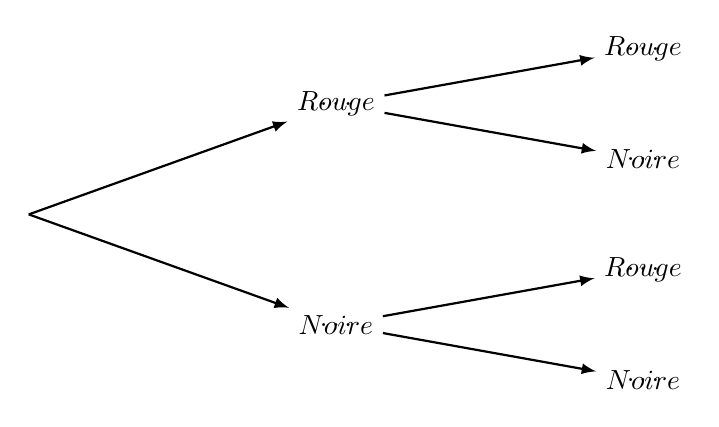
\begin{tikzpicture}[xscale=1.3,yscale=0.7]
% Styles (MODIFIABLES)
\tikzstyle{fleche}=[->,>=latex,thick]
% Dimensions (MODIFIABLES)
\def\DistanceInterNiveaux{3}
\def\DistanceInterFeuilles{2}
% Dimensions calculées (NON MODIFIABLES)
\def\NiveauA{(0)*\DistanceInterNiveaux}
\def\NiveauB{(1)*\DistanceInterNiveaux}
\def\NiveauC{(2)*\DistanceInterNiveaux}
\def\InterFeuilles{(-1)*\DistanceInterFeuilles}
% Noeuds (MODIFIABLES : Styles et Coefficients d'InterFeuilles)
\coordinate (R) at ({\NiveauA},{(1.5)*\InterFeuilles}) {};
\node (Ra) at ({\NiveauB},{(0.5)*\InterFeuilles}) {$Rouge$};
\node (Raa) at ({\NiveauC},{(0)*\InterFeuilles}) {$Rouge$};
\node (Rab) at ({\NiveauC},{(1)*\InterFeuilles}) {$Noire$};
\node (Rb) at ({\NiveauB},{(2.5)*\InterFeuilles}) {$Noire$};
\node (Rba) at ({\NiveauC},{(2)*\InterFeuilles}) {$Rouge$};
\node (Rbb) at ({\NiveauC},{(3)*\InterFeuilles}) {$Noire$};
% Arcs (MODIFIABLES : Styles)
\draw[fleche] (R)--(Ra) node {$\dots$};
\draw[fleche] (Ra)--(Raa) node {$\dots$};
\draw[fleche] (Ra)--(Rab) node {$\dots$};
\draw[fleche] (R)--(Rb) node {$\dots$};
\draw[fleche] (Rb)--(Rba) node {$\dots$};
\draw[fleche] (Rb)--(Rbb) node {$\dots$};
\end{tikzpicture}
\end{center}
\part Quelle est la probabilité que les deux boules obtenues soient rouge ? On donnera uniquement la formule permettant de calculer cette probabilité.
\part Quelle est la probabilité que les deux boules obtenues soient de la même couleur ? On donnera uniquement la formule permettant de calculer cette probabilité.
\end{parts}
\begin{solution}
\begin{parts}
\part \hfill
\begin{center}
% Racine à Gauche, développement vers la droite
\begin{tikzpicture}[xscale=1.3,yscale=0.7]
% Styles (MODIFIABLES)
\tikzstyle{fleche}=[->,>=latex,thick]
% Dimensions (MODIFIABLES)
\def\DistanceInterNiveaux{3}
\def\DistanceInterFeuilles{2}
% Dimensions calculées (NON MODIFIABLES)
\def\NiveauA{(0)*\DistanceInterNiveaux}
\def\NiveauB{(1)*\DistanceInterNiveaux}
\def\NiveauC{(2)*\DistanceInterNiveaux}
\def\InterFeuilles{(-1)*\DistanceInterFeuilles}
% Noeuds (MODIFIABLES : Styles et Coefficients d'InterFeuilles)
\coordinate (R) at ({\NiveauA},{(1.5)*\InterFeuilles}) {};
\node (Ra) at ({\NiveauB},{(0.5)*\InterFeuilles}) {$Rouge$};
\node (Raa) at ({\NiveauC},{(0)*\InterFeuilles}) {$Rouge$};
\node (Rab) at ({\NiveauC},{(1)*\InterFeuilles}) {$Noire$};
\node (Rb) at ({\NiveauB},{(2.5)*\InterFeuilles}) {$Noire$};
\node (Rba) at ({\NiveauC},{(2)*\InterFeuilles}) {$Rouge$};
\node (Rbb) at ({\NiveauC},{(3)*\InterFeuilles}) {$Noire$};
% Arcs (MODIFIABLES : Styles)
\draw[fleche] (R)--(Ra) node[midway,above] {$\dfrac{12}{18}$};
\draw[fleche] (Ra)--(Raa) node[midway,above] {$\dfrac{11}{17}$};
\draw[fleche] (Ra)--(Rab) node[midway,below] {$\dfrac{6}{17}$};
\draw[fleche] (R)--(Rb) node[midway,below] {$\dfrac{6}{18}$};
\draw[fleche] (Rb)--(Rba) node[midway,above] {$\dfrac{12}{17}$};
\draw[fleche] (Rb)--(Rbb) node[midway,below] {$\dfrac{5}{17}$};
\end{tikzpicture}
\end{center}
\part La probabilité est donnée par
\begin{equation*}
\dfrac{12}{18} \times \dfrac{11}{17}
\end{equation*}
\part La probabilité est donnée par
\begin{equation*}
\dfrac{12}{18} \times \dfrac{11}{17} + \dfrac{6}{18} \times \dfrac{5}{17}
\end{equation*}
\end{parts}
\end{solution}
\end{questions}
\newpage
\setcounter{page}{1}
\titleandname{}
\version{}
\begin{questions}
\question Dans une urne, il y a $8$ boules vertes et $6$ boules jaunes. On tire successivement deux boules de cette urne \textbf{sans remise}. On regarde la couleur des deux boules tirées.
\begin{parts}
\part Compléter l'arbre de probabilités ci-après avec les bonnes probabilités.
%:-+-+-+- Engendré par : http://math.et.info.free.fr/TikZ/Arbre/
\begin{center}
% Racine à Gauche, développement vers la droite
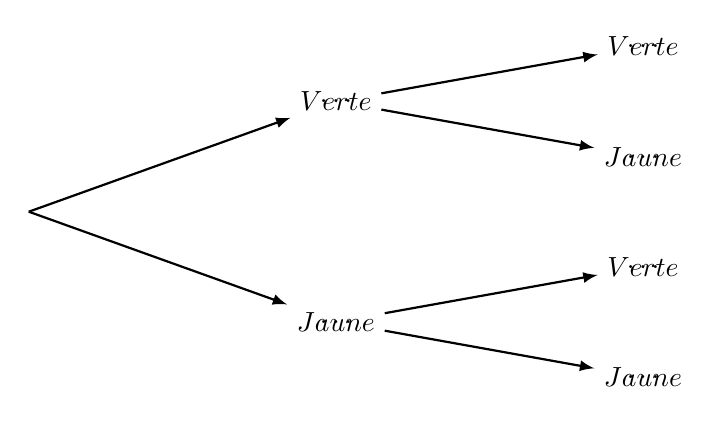
\begin{tikzpicture}[xscale=1.3,yscale=0.7]
% Styles (MODIFIABLES)
\tikzstyle{fleche}=[->,>=latex,thick]
% Dimensions (MODIFIABLES)
\def\DistanceInterNiveaux{3}
\def\DistanceInterFeuilles{2}
% Dimensions calculées (NON MODIFIABLES)
\def\NiveauA{(0)*\DistanceInterNiveaux}
\def\NiveauB{(1)*\DistanceInterNiveaux}
\def\NiveauC{(2)*\DistanceInterNiveaux}
\def\InterFeuilles{(-1)*\DistanceInterFeuilles}
% Noeuds (MODIFIABLES : Styles et Coefficients d'InterFeuilles)
\coordinate (R) at ({\NiveauA},{(1.5)*\InterFeuilles}) {};
\node (Ra) at ({\NiveauB},{(0.5)*\InterFeuilles}) {$Verte$};
\node (Raa) at ({\NiveauC},{(0)*\InterFeuilles}) {$Verte$};
\node (Rab) at ({\NiveauC},{(1)*\InterFeuilles}) {$Jaune$};
\node (Rb) at ({\NiveauB},{(2.5)*\InterFeuilles}) {$Jaune$};
\node (Rba) at ({\NiveauC},{(2)*\InterFeuilles}) {$Verte$};
\node (Rbb) at ({\NiveauC},{(3)*\InterFeuilles}) {$Jaune$};
% Arcs (MODIFIABLES : Styles)
\draw[fleche] (R)--(Ra) node {$\dots$};
\draw[fleche] (Ra)--(Raa) node {$\dots$};
\draw[fleche] (Ra)--(Rab) node {$\dots$};
\draw[fleche] (R)--(Rb) node {$\dots$};
\draw[fleche] (Rb)--(Rba) node {$\dots$};
\draw[fleche] (Rb)--(Rbb) node {$\dots$};
\end{tikzpicture}
\end{center}
\part Quelle est la probabilité que les deux boules obtenues soient jaunes ? On donnera uniquement la formule permettant de calculer cette probabilité.
\part Quelle est la probabilité que les deux boules obtenues soient de couleur différentes ? On donnera uniquement la formule permettant de calculer cette probabilité.
\end{parts}
\begin{solution}
\begin{parts}
\part \hfill
\begin{center}
% Racine à Gauche, développement vers la droite
\begin{tikzpicture}[xscale=1.3,yscale=0.7]
% Styles (MODIFIABLES)
\tikzstyle{fleche}=[->,>=latex,thick]
% Dimensions (MODIFIABLES)
\def\DistanceInterNiveaux{3}
\def\DistanceInterFeuilles{2}
% Dimensions calculées (NON MODIFIABLES)
\def\NiveauA{(0)*\DistanceInterNiveaux}
\def\NiveauB{(1)*\DistanceInterNiveaux}
\def\NiveauC{(2)*\DistanceInterNiveaux}
\def\InterFeuilles{(-1)*\DistanceInterFeuilles}
% Noeuds (MODIFIABLES : Styles et Coefficients d'InterFeuilles)
\coordinate (R) at ({\NiveauA},{(1.5)*\InterFeuilles}) {};
\node (Ra) at ({\NiveauB},{(0.5)*\InterFeuilles}) {$Verte$};
\node (Raa) at ({\NiveauC},{(0)*\InterFeuilles}) {$Verte$};
\node (Rab) at ({\NiveauC},{(1)*\InterFeuilles}) {$Jaune$};
\node (Rb) at ({\NiveauB},{(2.5)*\InterFeuilles}) {$Jaune$};
\node (Rba) at ({\NiveauC},{(2)*\InterFeuilles}) {$Verte$};
\node (Rbb) at ({\NiveauC},{(3)*\InterFeuilles}) {$Jaune$};
% Arcs (MODIFIABLES : Styles)
\draw[fleche] (R)--(Ra) node[midway,above] {$\dfrac{8}{14}$};
\draw[fleche] (Ra)--(Raa) node[midway,above] {$\dfrac{7}{13}$};
\draw[fleche] (Ra)--(Rab) node[midway,below] {$\dfrac{6}{13}$};
\draw[fleche] (R)--(Rb) node[midway,below] {$\dfrac{6}{14}$};
\draw[fleche] (Rb)--(Rba) node[midway,above] {$\dfrac{8}{13}$};
\draw[fleche] (Rb)--(Rbb) node[midway,below] {$\dfrac{5}{13}$};
\end{tikzpicture}
\end{center}
\part La probabilité est donnée par
\begin{equation*}
\dfrac{6}{14} \times \dfrac{5}{13}
\end{equation*}
\part La probabilité est donnée par
\begin{equation*}
\dfrac{8}{14} \times \dfrac{6}{13} + \dfrac{6}{14} \times \dfrac{8}{13}
\end{equation*}
\end{parts}
\end{solution}
\end{questions}
\end{document}